\chapter{Scatter Plots}\label{scatter-plots}

In this part, we will work towards creating the scatterplot below. We
will take you from a basic scatterplot and explain all the
customisations we add to the code step-by-step.

\begin{center}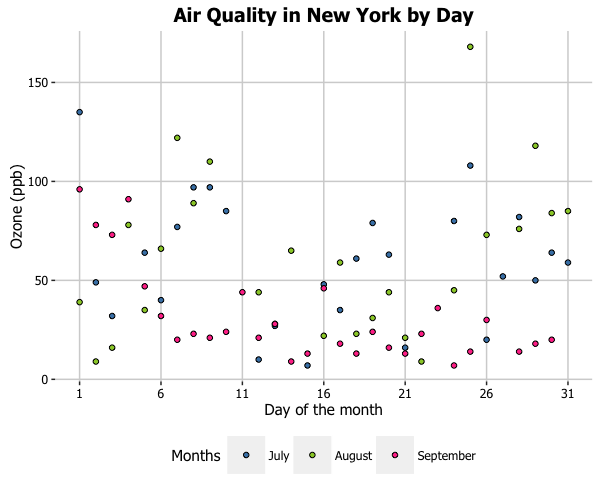
\includegraphics[width=0.55\linewidth]{0_all_posts_pdf/scatter_finalgraph-1} \end{center}

The first thing to do is load in the data, as below:

\begin{Shaded}
\begin{Highlighting}[]
\KeywordTok{library}\NormalTok{(ggplot2)}
\KeywordTok{library}\NormalTok{(ggthemes)}
\KeywordTok{library}\NormalTok{(extrafont)}
\KeywordTok{library}\NormalTok{(datasets)}
\KeywordTok{data}\NormalTok{(airquality)}
\end{Highlighting}
\end{Shaded}

We will then trim the data down to the final three months and turn the
\texttt{Month} variable into a labelled factor variable. We end up with
a new dataset called \texttt{aq\_trim}.

\begin{Shaded}
\begin{Highlighting}[]
\NormalTok{aq_trim <-}\StringTok{ }\NormalTok{airquality[}\KeywordTok{which}\NormalTok{(airquality$Month ==}\StringTok{ }\DecValTok{7} \NormalTok{|}
\NormalTok{airquality$Month ==}\StringTok{ }\DecValTok{8} \NormalTok{|}
\NormalTok{airquality$Month ==}\StringTok{ }\DecValTok{9}\NormalTok{), ]}
\NormalTok{aq_trim$Month <-}\StringTok{ }\KeywordTok{factor}\NormalTok{(aq_trim$Month, }
\DataTypeTok{labels =} \KeywordTok{c}\NormalTok{(}\StringTok{"July"}\NormalTok{, }\StringTok{"August"}\NormalTok{, }\StringTok{"September"}\NormalTok{))}
\end{Highlighting}
\end{Shaded}

\section{Basic scatterplot}\label{basic-scatterplot}

In order to initialise a scatterplot we tell ggplot that
\texttt{aq\_trim} is our data, and specify that our x-axis plots the
\texttt{Day} variable and our y-axis plots the \texttt{Ozone} variable.
We then instruct ggplot to render this as a scatterplot by adding the
\texttt{geom\_point()} option.

\begin{Shaded}
\begin{Highlighting}[]
\NormalTok{p5 <-}\StringTok{ }\KeywordTok{ggplot}\NormalTok{(aq_trim, }\KeywordTok{aes}\NormalTok{(}\DataTypeTok{x =} \NormalTok{Day, }\DataTypeTok{y =} \NormalTok{Ozone)) +}\StringTok{ }
\StringTok{      }\KeywordTok{geom_point}\NormalTok{()}
\NormalTok{p5}
\end{Highlighting}
\end{Shaded}

\begin{center}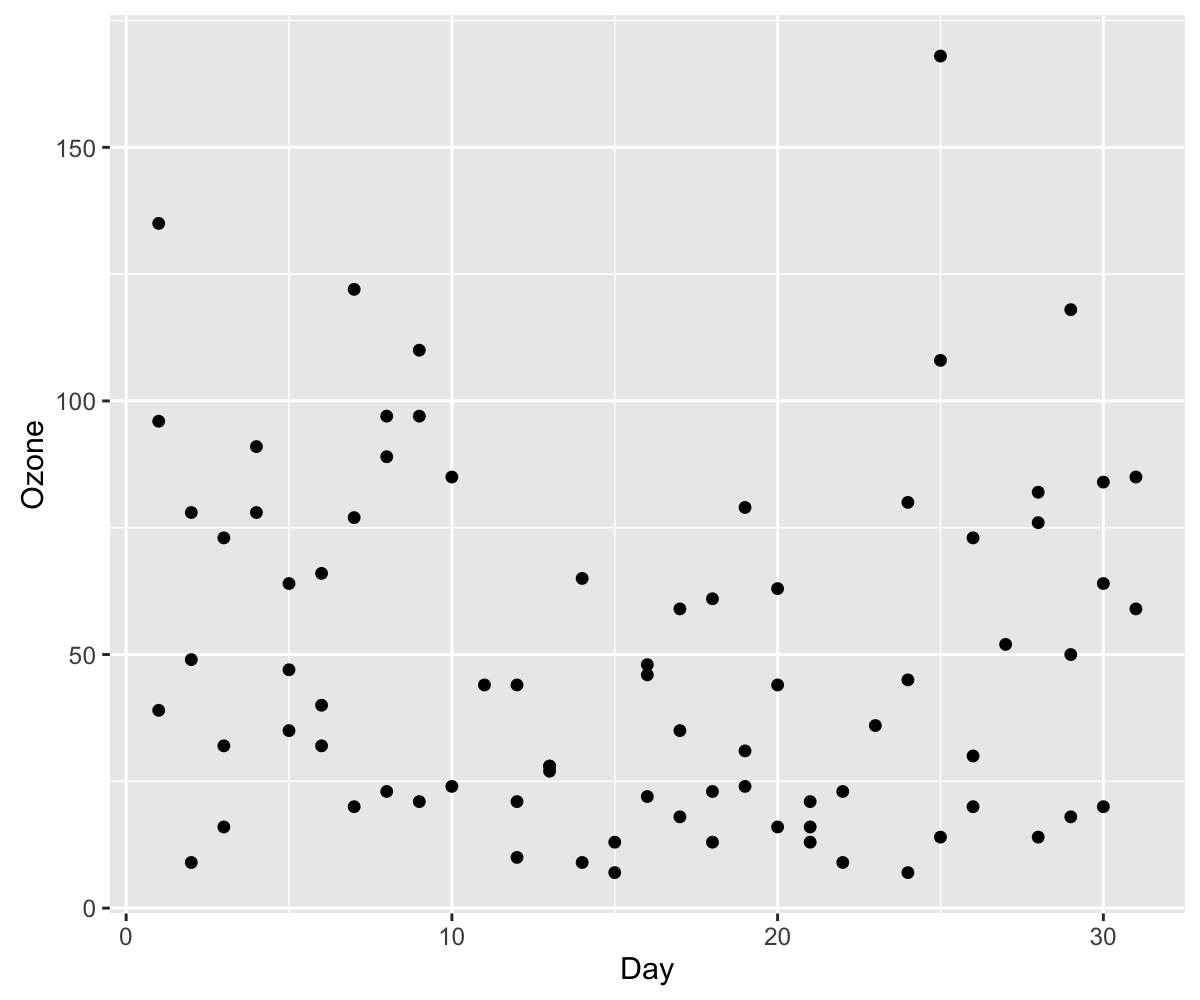
\includegraphics[width=0.55\linewidth]{0_all_posts_pdf/scatter_1-1} \end{center}

\section{Changing the shape of the data
points}\label{changing-the-shape-of-the-data-points}

Perhaps we want the data points to be a different shape than a solid
circle. We can change these by adding the \texttt{shape} argument to
\texttt{geom\_point}. An explanation of the allowed arguments for shape
are described in
\href{http://sape.inf.usi.ch/quick-reference/ggplot2/shape}{this
article}. In this case, we will use shape 21, which is a circle that
allows different colours for the outline and fill.

\begin{Shaded}
\begin{Highlighting}[]
\NormalTok{p5 <-}\StringTok{ }\KeywordTok{ggplot}\NormalTok{(aq_trim, }\KeywordTok{aes}\NormalTok{(}\DataTypeTok{x =} \NormalTok{Day, }\DataTypeTok{y =} \NormalTok{Ozone)) +}\StringTok{ }\KeywordTok{geom_point}\NormalTok{(}\DataTypeTok{shape =} \DecValTok{21}\NormalTok{)}
\NormalTok{p5}
\end{Highlighting}
\end{Shaded}

\begin{center}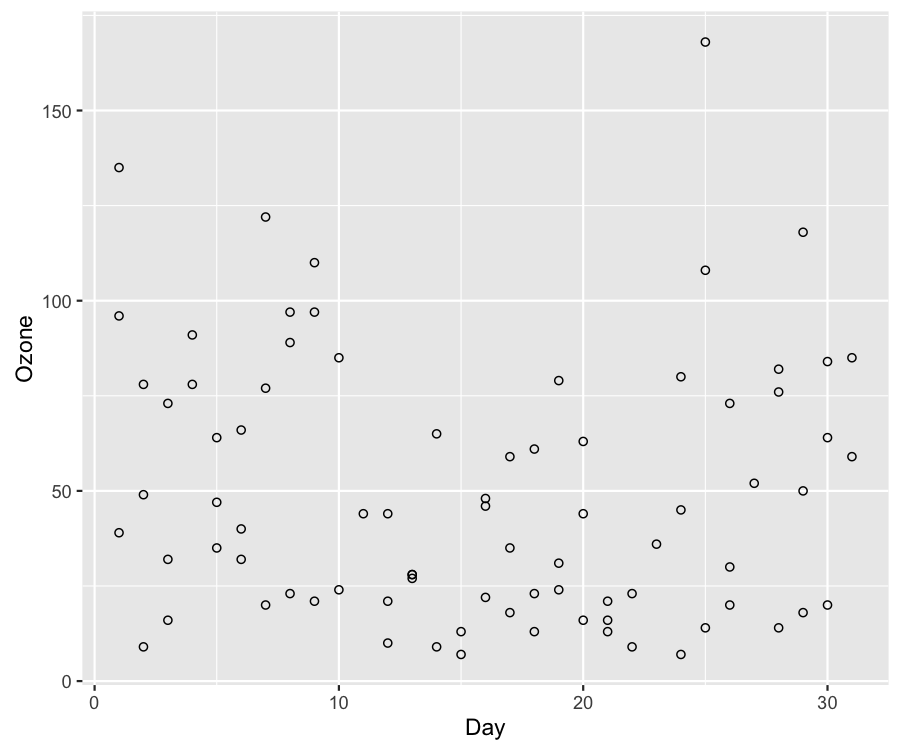
\includegraphics[width=0.55\linewidth]{0_all_posts_pdf/scatter_2-1} \end{center}

\section{Adjusting the axis scales}\label{adjusting-the-axis-scales}

To change the x-axis tick marks, we use the
\texttt{scale\_x\_continuous} option. Similarly, to change the y-axis we
use the \texttt{scale\_y\_continuous} option. Here we will change the
x-axis to every 5 days, rather than 10, and change the range from 1 to
31 (as 0 is not a valid value for this variable).

\begin{Shaded}
\begin{Highlighting}[]
\NormalTok{p5 <-}\StringTok{ }\NormalTok{p5 +}\StringTok{ }\KeywordTok{scale_x_continuous}\NormalTok{(}\DataTypeTok{breaks =} \KeywordTok{seq}\NormalTok{(}\DecValTok{1}\NormalTok{, }\DecValTok{31}\NormalTok{, }\DecValTok{5}\NormalTok{))}
\NormalTok{p5}
\end{Highlighting}
\end{Shaded}

\begin{center}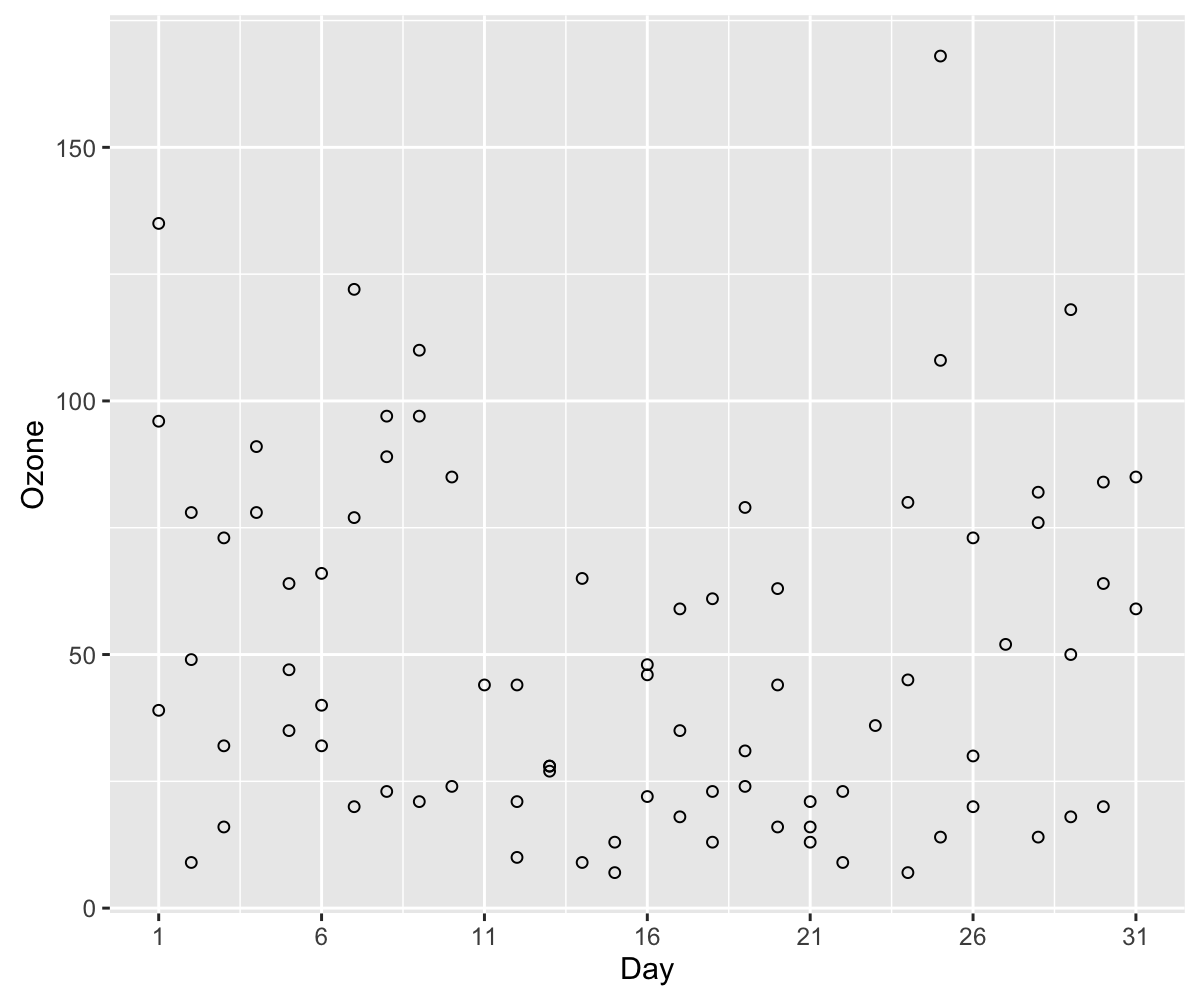
\includegraphics[width=0.55\linewidth]{0_all_posts_pdf/scatter_3-1} \end{center}

\section{Adjusting axis labels \& adding
title}\label{adjusting-axis-labels-adding-title-3}

To add a title, we include the option \texttt{ggtitle} and include the
name of the graph as a string argument. To change the axis names we add
\texttt{x} and \texttt{y} arguments to the \texttt{labs} command.

\begin{Shaded}
\begin{Highlighting}[]
\NormalTok{p5 <-}\StringTok{ }\NormalTok{p5 +}\StringTok{ }\KeywordTok{ggtitle}\NormalTok{(}\StringTok{"Air Quality in New York by Day"}\NormalTok{) +}\StringTok{ }
\StringTok{      }\KeywordTok{labs}\NormalTok{(}\DataTypeTok{x =} \StringTok{"Day of the month"}\NormalTok{, }\DataTypeTok{y =} \StringTok{"Ozone (ppb)"}\NormalTok{) }
\NormalTok{p5}
\end{Highlighting}
\end{Shaded}

\begin{center}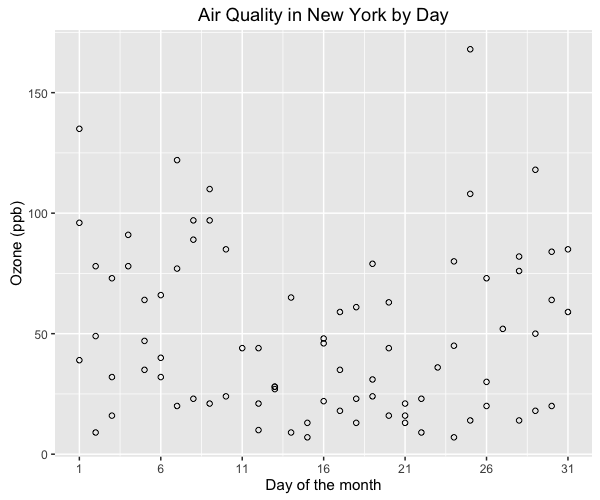
\includegraphics[width=0.55\linewidth]{0_all_posts_pdf/scatter_4-1} \end{center}

\section{Adjusting the colour
palette}\label{adjusting-the-colour-palette}

There are a few options for adjusting the colour. The most simple is to
make every point one fixed colour. You can reference colours by name,
with the full list of colours recognised by R
\href{http://www.stat.columbia.edu/~tzheng/files/Rcolor.pdf}{here}.
Let's try making the outline \texttt{mediumvioletred} and the fill
\texttt{springgreen}.

\begin{Shaded}
\begin{Highlighting}[]
\NormalTok{p5 <-}\StringTok{ }\KeywordTok{ggplot}\NormalTok{(aq_trim, }\KeywordTok{aes}\NormalTok{(}\DataTypeTok{x =} \NormalTok{Day, }\DataTypeTok{y =} \NormalTok{Ozone)) +}\StringTok{ }
\StringTok{      }\KeywordTok{geom_point}\NormalTok{(}\DataTypeTok{shape =} \DecValTok{21}\NormalTok{, }\DataTypeTok{colour =} \StringTok{"mediumvioletred"}\NormalTok{, }\DataTypeTok{fill =} \StringTok{"springgreen"}\NormalTok{) +}
\StringTok{      }\KeywordTok{ggtitle}\NormalTok{(}\StringTok{"Air Quality in New York by Day"}\NormalTok{) +}\StringTok{ }
\StringTok{      }\KeywordTok{labs}\NormalTok{(}\DataTypeTok{x =} \StringTok{"Day of the month"}\NormalTok{, }\DataTypeTok{y =} \StringTok{"Ozone (ppb)"}\NormalTok{) +}
\StringTok{      }\KeywordTok{scale_x_continuous}\NormalTok{(}\DataTypeTok{breaks =} \KeywordTok{seq}\NormalTok{(}\DecValTok{1}\NormalTok{, }\DecValTok{31}\NormalTok{, }\DecValTok{5}\NormalTok{)) }
\NormalTok{p5}
\end{Highlighting}
\end{Shaded}

\begin{center}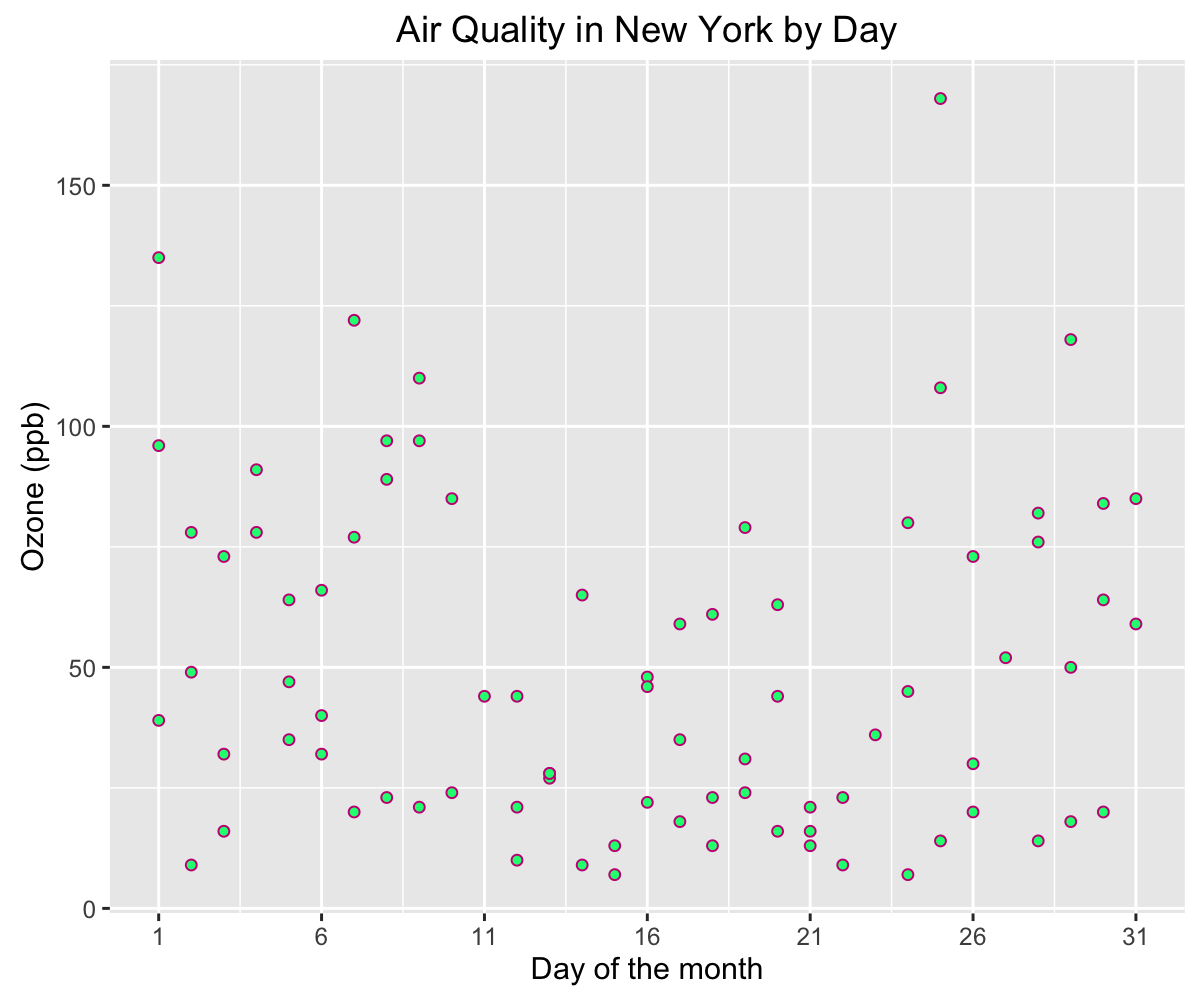
\includegraphics[width=0.55\linewidth]{0_all_posts_pdf/scatter_5-1} \end{center}

You can change the colours using specific HEX codes instead. Here we
have made the outline \#000000 (black) and the fill ``\#40b8d0 (vivid
cyan).

\begin{Shaded}
\begin{Highlighting}[]
\NormalTok{p5 <-}\StringTok{ }\KeywordTok{ggplot}\NormalTok{(aq_trim, }\KeywordTok{aes}\NormalTok{(}\DataTypeTok{x =} \NormalTok{Day, }\DataTypeTok{y =} \NormalTok{Ozone)) +}\StringTok{ }
\StringTok{      }\KeywordTok{geom_point}\NormalTok{(}\DataTypeTok{shape =} \DecValTok{21}\NormalTok{, }\DataTypeTok{colour =} \StringTok{"#000000"}\NormalTok{, }\DataTypeTok{fill =} \StringTok{"#40b8d0"}\NormalTok{) +}
\StringTok{      }\KeywordTok{ggtitle}\NormalTok{(}\StringTok{"Air Quality in New York by Day"}\NormalTok{) +}\StringTok{ }
\StringTok{      }\KeywordTok{labs}\NormalTok{(}\DataTypeTok{x =} \StringTok{"Day of the month"}\NormalTok{, }\DataTypeTok{y =} \StringTok{"Ozone (ppb)"}\NormalTok{) +}
\StringTok{      }\KeywordTok{scale_x_continuous}\NormalTok{(}\DataTypeTok{breaks =} \KeywordTok{seq}\NormalTok{(}\DecValTok{1}\NormalTok{, }\DecValTok{31}\NormalTok{, }\DecValTok{5}\NormalTok{))}
\NormalTok{p5}
\end{Highlighting}
\end{Shaded}

\begin{center}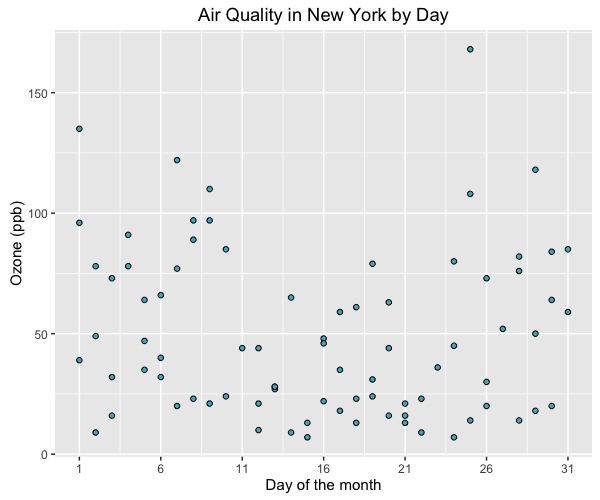
\includegraphics[width=0.55\linewidth]{0_all_posts_pdf/scatter_6-1} \end{center}

You can also change the colour of the data points according to the
levels of another variable. This can be done either as a continuous
gradient, or as a levels of a factor variable. Let's change the colour
by the values of temperature:

\begin{Shaded}
\begin{Highlighting}[]
\NormalTok{p5 <-}\StringTok{ }\KeywordTok{ggplot}\NormalTok{(aq_trim, }\KeywordTok{aes}\NormalTok{(}\DataTypeTok{x =} \NormalTok{Day, }\DataTypeTok{y =} \NormalTok{Ozone, }\DataTypeTok{fill =} \NormalTok{Temp)) +}\StringTok{ }
\StringTok{      }\KeywordTok{geom_point}\NormalTok{(}\DataTypeTok{shape =} \DecValTok{21}\NormalTok{) +}
\StringTok{      }\KeywordTok{ggtitle}\NormalTok{(}\StringTok{"Air Quality in New York by Day"}\NormalTok{) +}\StringTok{ }
\StringTok{      }\KeywordTok{labs}\NormalTok{(}\DataTypeTok{x =} \StringTok{"Day of the month"}\NormalTok{, }\DataTypeTok{y =} \StringTok{"Ozone (ppb)"}\NormalTok{) +}
\StringTok{      }\KeywordTok{scale_x_continuous}\NormalTok{(}\DataTypeTok{breaks =} \KeywordTok{seq}\NormalTok{(}\DecValTok{1}\NormalTok{, }\DecValTok{31}\NormalTok{, }\DecValTok{5}\NormalTok{))}
\NormalTok{p5}
\end{Highlighting}
\end{Shaded}

\begin{center}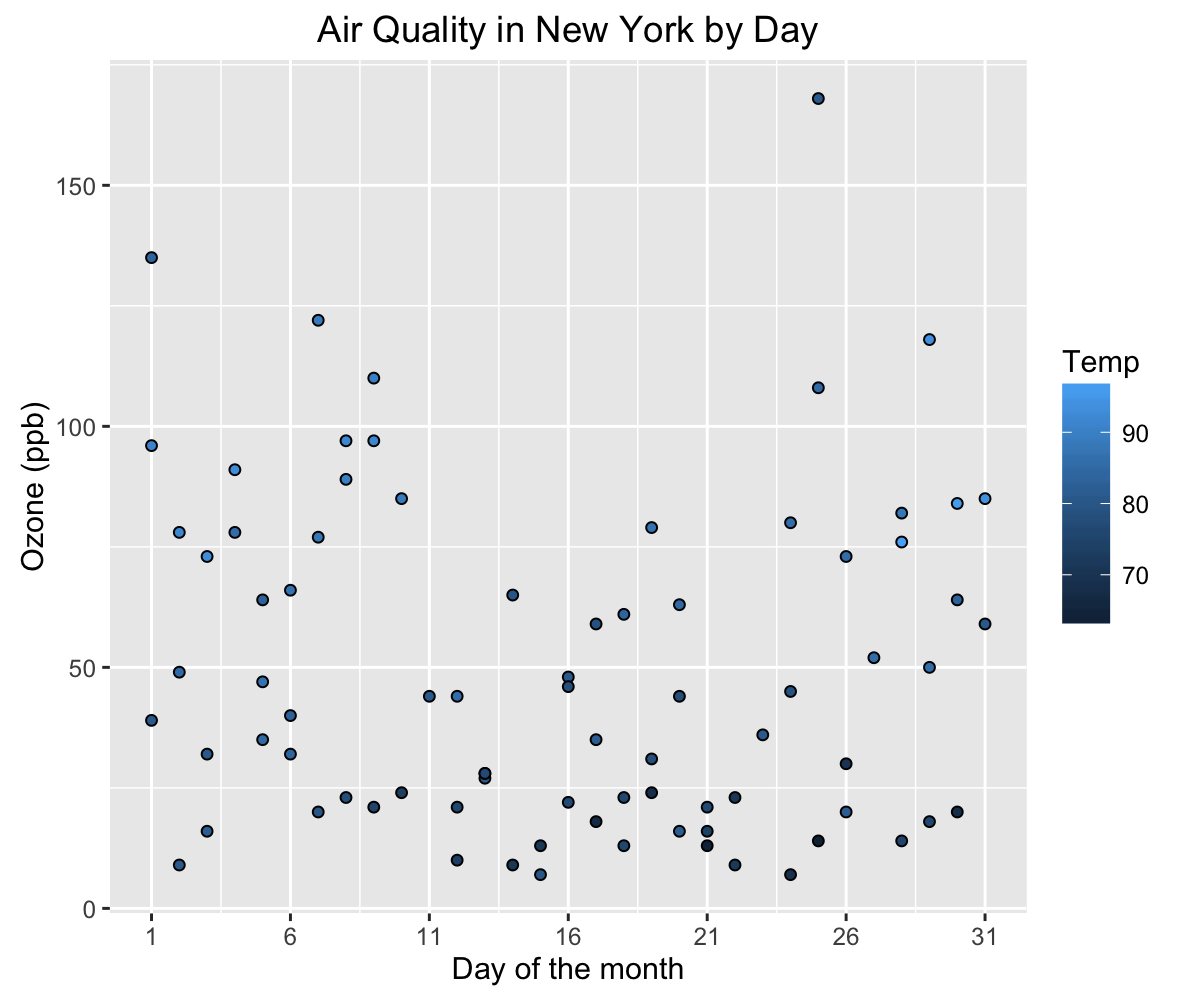
\includegraphics[width=0.55\linewidth]{0_all_posts_pdf/scatter_7-1} \end{center}

We can change the gradient's colours by adding the
\texttt{scale\_fill\_continuous} option. The \texttt{low} and
\texttt{high} arguments specify the range of colours the gradient should
transition between.

\begin{Shaded}
\begin{Highlighting}[]
\NormalTok{p5 <-}\StringTok{  }\NormalTok{p5 +}\StringTok{ }\KeywordTok{scale_fill_continuous}\NormalTok{(}\DataTypeTok{low =} \StringTok{"plum1"}\NormalTok{, }\DataTypeTok{high =} \StringTok{"purple4"}\NormalTok{)}
\NormalTok{p5}
\end{Highlighting}
\end{Shaded}

\begin{center}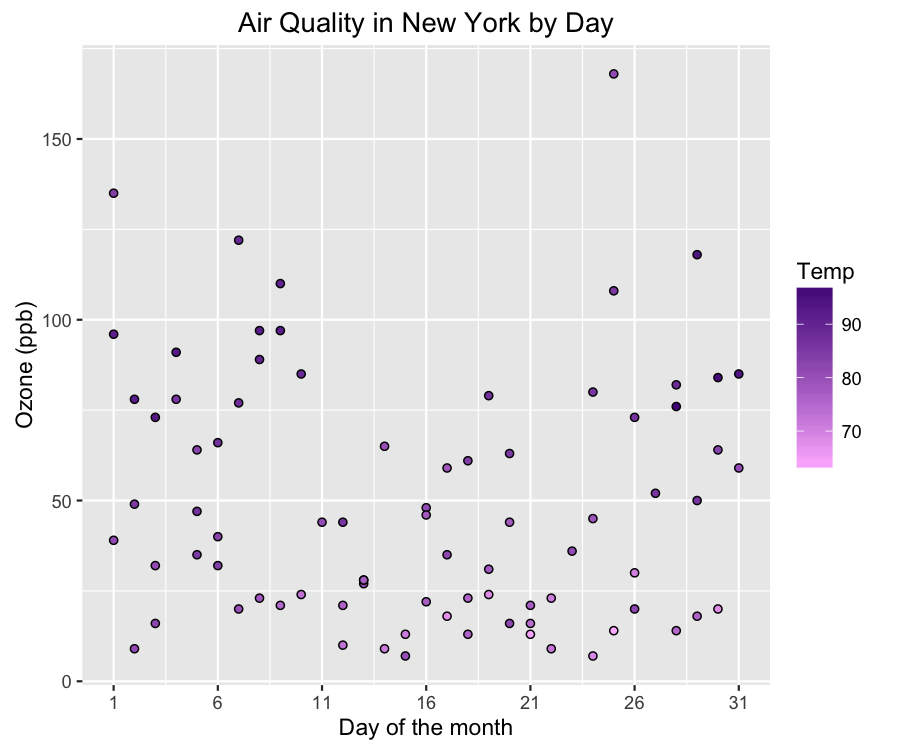
\includegraphics[width=0.55\linewidth]{0_all_posts_pdf/scatter_8-1} \end{center}

We can see that higher temperatures seem to have higher ozone levels.

Let's now change the colours of the data points by a factor variable,
\texttt{Month}.

\begin{Shaded}
\begin{Highlighting}[]
\NormalTok{p5 <-}\StringTok{ }\KeywordTok{ggplot}\NormalTok{(aq_trim, }\KeywordTok{aes}\NormalTok{(}\DataTypeTok{x =} \NormalTok{Day, }\DataTypeTok{y =} \NormalTok{Ozone, }\DataTypeTok{fill =} \NormalTok{Month)) +}\StringTok{ }
\StringTok{      }\KeywordTok{geom_point}\NormalTok{(}\DataTypeTok{shape =} \DecValTok{21}\NormalTok{) +}
\StringTok{      }\KeywordTok{ggtitle}\NormalTok{(}\StringTok{"Air Quality in New York by Day"}\NormalTok{) +}\StringTok{ }
\StringTok{      }\KeywordTok{labs}\NormalTok{(}\DataTypeTok{x =} \StringTok{"Day of the month"}\NormalTok{, }\DataTypeTok{y =} \StringTok{"Ozone (ppb)"}\NormalTok{) +}
\StringTok{      }\KeywordTok{scale_x_continuous}\NormalTok{(}\DataTypeTok{breaks =} \KeywordTok{seq}\NormalTok{(}\DecValTok{1}\NormalTok{, }\DecValTok{31}\NormalTok{, }\DecValTok{5}\NormalTok{))}
\NormalTok{p5}
\end{Highlighting}
\end{Shaded}

\begin{center}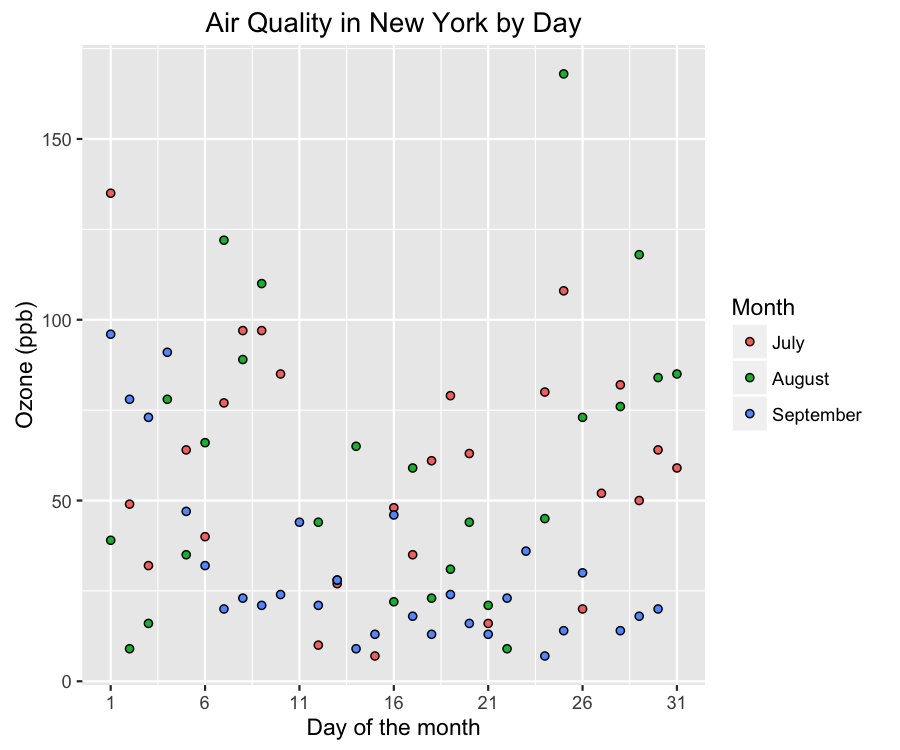
\includegraphics[width=0.55\linewidth]{0_all_posts_pdf/scatter_9-1} \end{center}

Again, we can change the colours of these data points, this time using
\texttt{scale\_fill\_manual}.

\begin{Shaded}
\begin{Highlighting}[]
\NormalTok{fill =}\StringTok{ }\KeywordTok{c}\NormalTok{(}\StringTok{"steelblue"}\NormalTok{, }\StringTok{"yellowgreen"}\NormalTok{, }\StringTok{"violetred1"}\NormalTok{)}

\NormalTok{p5 <-}\StringTok{ }\NormalTok{p5 +}\StringTok{ }\KeywordTok{scale_fill_manual}\NormalTok{(}\DataTypeTok{values =} \NormalTok{fill)}
\NormalTok{p5}
\end{Highlighting}
\end{Shaded}

\begin{center}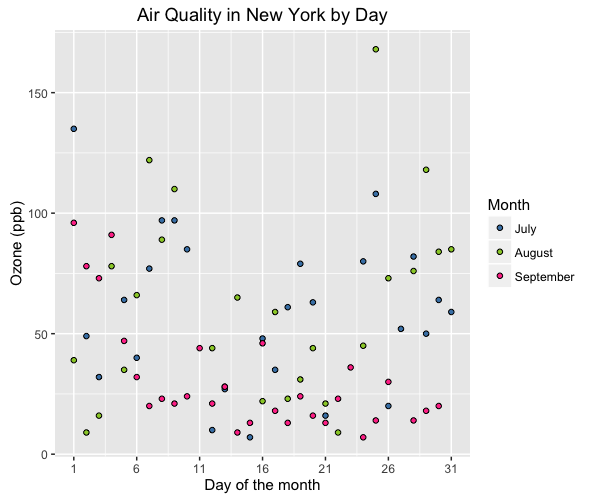
\includegraphics[width=0.55\linewidth]{0_all_posts_pdf/scatter_10-1} \end{center}

\section{Adjusting legend
position}\label{adjusting-legend-position-3}

To adjust the position of the legend from the default spot of right of
the graph, we add the \texttt{theme} option and specify the
\texttt{legend.position\ =\ "bottom"} argument. We can also change the
legend shape using the \texttt{legend.direction\ =\ "horizontal"}
argument.

\begin{Shaded}
\begin{Highlighting}[]
\NormalTok{p5 <-}\StringTok{ }\NormalTok{p5 +}\StringTok{ }\KeywordTok{theme}\NormalTok{(}\DataTypeTok{legend.position =} \StringTok{"bottom"}\NormalTok{, }\DataTypeTok{legend.direction =} \StringTok{"horizontal"}\NormalTok{)}
\NormalTok{p5}
\end{Highlighting}
\end{Shaded}

\begin{center}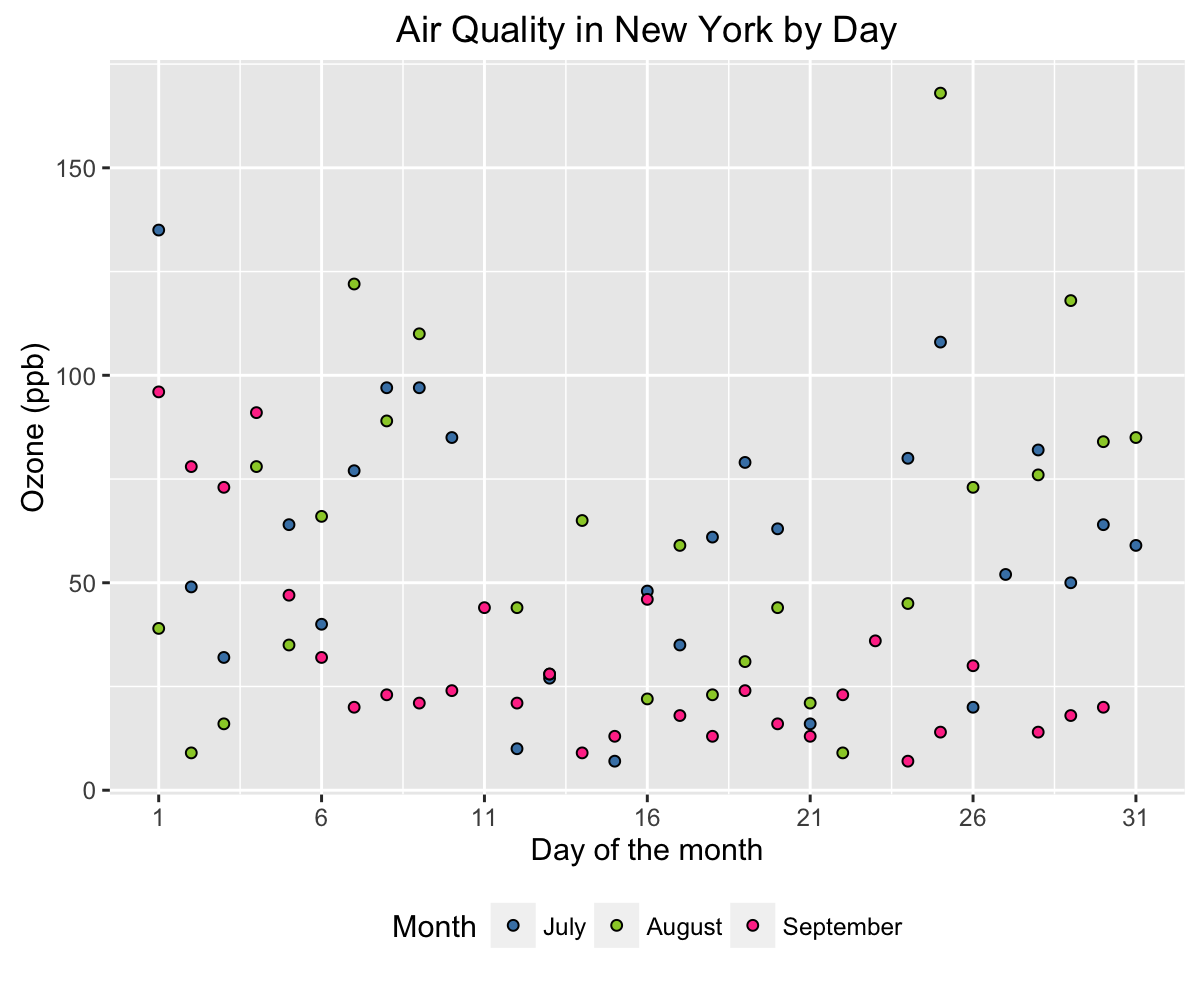
\includegraphics[width=0.55\linewidth]{0_all_posts_pdf/scatter_11-1} \end{center}

\section{Using the white theme}\label{using-the-white-theme-4}

As explained in the previous posts, we can also change the overall look
of the plot using themes. We'll start using a simple theme customisation
by adding \texttt{theme\_bw()} after \texttt{ggplot()}. As you can see,
we can further tweak the graph using the \texttt{theme} option, which
we've used so far to change the legend.

\begin{Shaded}
\begin{Highlighting}[]
\NormalTok{p5 <-}\StringTok{ }\KeywordTok{ggplot}\NormalTok{(aq_trim, }\KeywordTok{aes}\NormalTok{(}\DataTypeTok{x =} \NormalTok{Day, }\DataTypeTok{y =} \NormalTok{Ozone, }\DataTypeTok{fill =} \NormalTok{Month)) +}\StringTok{ }\KeywordTok{theme_bw}\NormalTok{() +}
\StringTok{      }\KeywordTok{geom_point}\NormalTok{(}\DataTypeTok{shape =} \DecValTok{21}\NormalTok{) +}
\StringTok{      }\KeywordTok{ggtitle}\NormalTok{(}\StringTok{"Air Quality in New York by Day"}\NormalTok{) +}\StringTok{ }
\StringTok{      }\KeywordTok{labs}\NormalTok{(}\DataTypeTok{x =} \StringTok{"Day of the month"}\NormalTok{, }\DataTypeTok{y =} \StringTok{"Ozone (ppb)"}\NormalTok{, }\DataTypeTok{fill =} \StringTok{"Months"}\NormalTok{) +}
\StringTok{      }\KeywordTok{scale_x_continuous}\NormalTok{(}\DataTypeTok{breaks =} \KeywordTok{seq}\NormalTok{(}\DecValTok{1}\NormalTok{, }\DecValTok{31}\NormalTok{, }\DecValTok{5}\NormalTok{)) +}
\StringTok{      }\KeywordTok{scale_fill_manual}\NormalTok{(}\DataTypeTok{values =} \NormalTok{fill) +}
\StringTok{      }\KeywordTok{scale_size}\NormalTok{(}\DataTypeTok{range =} \KeywordTok{c}\NormalTok{(}\DecValTok{1}\NormalTok{, }\DecValTok{10}\NormalTok{)) +}
\StringTok{      }\KeywordTok{theme}\NormalTok{(}\DataTypeTok{legend.position=}\StringTok{"bottom"}\NormalTok{, }\DataTypeTok{legend.direction=}\StringTok{"horizontal"}\NormalTok{)}
\NormalTok{p5}
\end{Highlighting}
\end{Shaded}

\begin{center}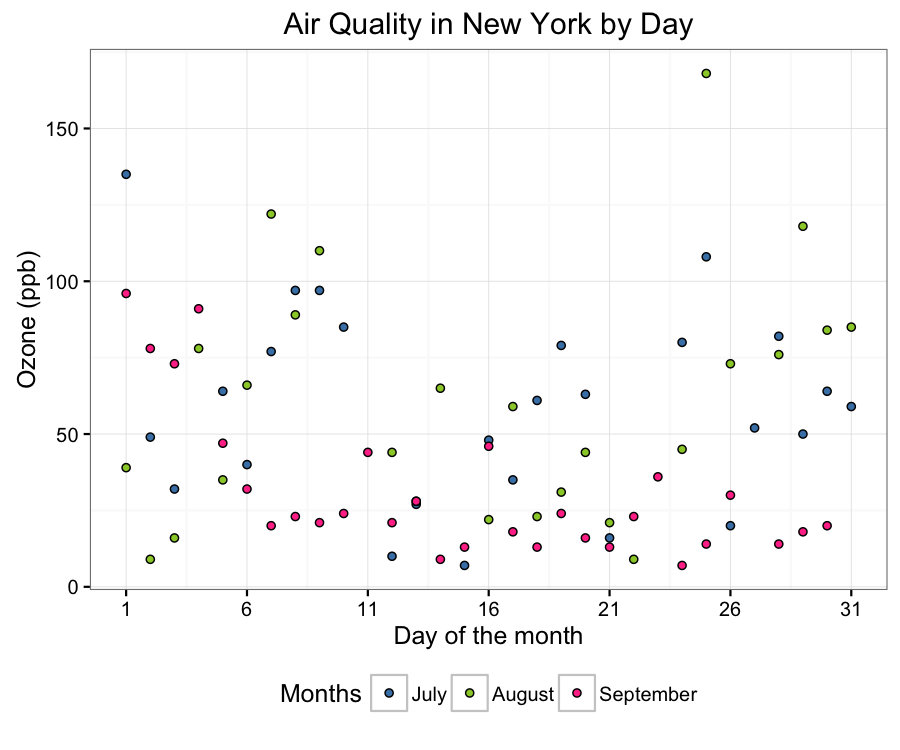
\includegraphics[width=0.55\linewidth]{0_all_posts_pdf/scatter_12-1} \end{center}

\section{Creating an XKCD style
chart}\label{creating-an-xkcd-style-chart-4}

Of course, you may want to create your own themes as well.
\texttt{ggplot2} allows for a very high degree of customisation,
including allowing you to use imported fonts. Below is an example of a
theme Mauricio was able to create which mimics the visual style of
\href{http://xkcd.com/}{XKCD}. In order to create this chart, you first
need to import the XKCD font, install it on your machine and load it
into R using the \texttt{extrafont} package. These instructions are
taken from
\href{https://www.google.com.au/url?sa=t\&rct=j\&q=\&esrc=s\&source=web\&cd=1\&ved=0ahUKEwiWzafchdPJAhVBpJQKHe_LDT8QFggbMAA\&url=https\%3A\%2F\%2Fcran.r-project.org\%2Fweb\%2Fpackages\%2Fxkcd\%2Fvignettes\%2Fxkcd-intro.pdf\&usg=AFQjCNE-KciGY14e-Q1buYIVmTFC0ht__Q\&sig2=DZUwkvIHwfNWtTtkcz94jg}{here}:

\begin{Shaded}
\begin{Highlighting}[]
\KeywordTok{library}\NormalTok{(extrafont)}

\KeywordTok{download.file}\NormalTok{(}\StringTok{"http://simonsoftware.se/other/xkcd.ttf"}\NormalTok{, }\DataTypeTok{dest=}\StringTok{"xkcd.ttf"}\NormalTok{, }
	\DataTypeTok{mode=}\StringTok{"wb"}\NormalTok{)}
\KeywordTok{system}\NormalTok{(}\StringTok{"mkdir ~/.fonts"}\NormalTok{)}
\KeywordTok{system}\NormalTok{(}\StringTok{"cp xkcd.ttf  ~/.fonts"}\NormalTok{)}
\KeywordTok{font_import}\NormalTok{(}\DataTypeTok{paths =} \StringTok{"~/.fonts"}\NormalTok{, }\DataTypeTok{pattern=}\StringTok{"[X/x]kcd"}\NormalTok{)}
\KeywordTok{fonts}\NormalTok{()}
\KeywordTok{loadfonts}\NormalTok{()}
\end{Highlighting}
\end{Shaded}

You can then create your graph:

\begin{Shaded}
\begin{Highlighting}[]
\NormalTok{fill <-}\StringTok{ }\KeywordTok{c}\NormalTok{(}\StringTok{"#56B4E9"}\NormalTok{, }\StringTok{"#F0E442"}\NormalTok{, }\StringTok{"violetred1"}\NormalTok{)}

\NormalTok{p5 <-}\StringTok{ }\KeywordTok{ggplot}\NormalTok{(aq_trim, }\KeywordTok{aes}\NormalTok{(}\DataTypeTok{x =} \NormalTok{Day, }\DataTypeTok{y =} \NormalTok{Ozone, }\DataTypeTok{fill =} \NormalTok{Month)) +}\StringTok{ }
\StringTok{      }\KeywordTok{geom_point}\NormalTok{(}\DataTypeTok{shape =} \DecValTok{21}\NormalTok{) +}
\StringTok{      }\KeywordTok{ggtitle}\NormalTok{(}\StringTok{"Air Quality in New York by Day"}\NormalTok{) +}\StringTok{ }
\StringTok{      }\KeywordTok{labs}\NormalTok{(}\DataTypeTok{x =} \StringTok{"Day of the month"}\NormalTok{, }\DataTypeTok{y =} \StringTok{"Ozone (ppb)"}\NormalTok{, }\DataTypeTok{fill =} \StringTok{"Months"}\NormalTok{) +}
\StringTok{      }\KeywordTok{scale_x_continuous}\NormalTok{(}\DataTypeTok{breaks =} \KeywordTok{seq}\NormalTok{(}\DecValTok{1}\NormalTok{, }\DecValTok{31}\NormalTok{, }\DecValTok{5}\NormalTok{)) +}
\StringTok{      }\KeywordTok{scale_fill_manual}\NormalTok{(}\DataTypeTok{values =} \NormalTok{fill) +}
\StringTok{      }\KeywordTok{scale_size}\NormalTok{(}\DataTypeTok{range =} \KeywordTok{c}\NormalTok{(}\DecValTok{1}\NormalTok{, }\DecValTok{10}\NormalTok{)) +}
\StringTok{      }\KeywordTok{theme}\NormalTok{(}\DataTypeTok{axis.line.x =} \KeywordTok{element_line}\NormalTok{(}\DataTypeTok{size=}\DecValTok{1}\NormalTok{, }\DataTypeTok{colour =} \StringTok{"black"}\NormalTok{),}
\StringTok{        }\DataTypeTok{axis.line.y =} \KeywordTok{element_line}\NormalTok{(}\DataTypeTok{size=}\DecValTok{1}\NormalTok{, }\DataTypeTok{colour =} \StringTok{"black"}\NormalTok{),}
\StringTok{        }\DataTypeTok{axis.text.x=}\KeywordTok{element_text}\NormalTok{(}\DataTypeTok{colour=}\StringTok{"black"}\NormalTok{, }\DataTypeTok{size =} \DecValTok{10}\NormalTok{), }
\StringTok{        }\DataTypeTok{axis.text.y=}\KeywordTok{element_text}\NormalTok{(}\DataTypeTok{colour=}\StringTok{"black"}\NormalTok{, }\DataTypeTok{size =} \DecValTok{10}\NormalTok{), }
\StringTok{        }\DataTypeTok{legend.position=}\StringTok{"bottom"}\NormalTok{, }\DataTypeTok{legend.direction=}\StringTok{"horizontal"}\NormalTok{,}
\StringTok{        }\DataTypeTok{panel.grid.major =} \KeywordTok{element_blank}\NormalTok{(),}
\StringTok{        }\DataTypeTok{panel.grid.minor =} \KeywordTok{element_blank}\NormalTok{(), }
\StringTok{        }\DataTypeTok{panel.border =} \KeywordTok{element_blank}\NormalTok{(),}
\StringTok{        }\DataTypeTok{panel.background =} \KeywordTok{element_blank}\NormalTok{(),}
\StringTok{        }\DataTypeTok{plot.title=}\KeywordTok{element_text}\NormalTok{(}\DataTypeTok{family=}\StringTok{"xkcd-Regular"}\NormalTok{), }
\StringTok{        }\DataTypeTok{text=}\KeywordTok{element_text}\NormalTok{(}\DataTypeTok{family=}\StringTok{"xkcd-Regular"}\NormalTok{)) }
\NormalTok{p5}
\end{Highlighting}
\end{Shaded}

\begin{center}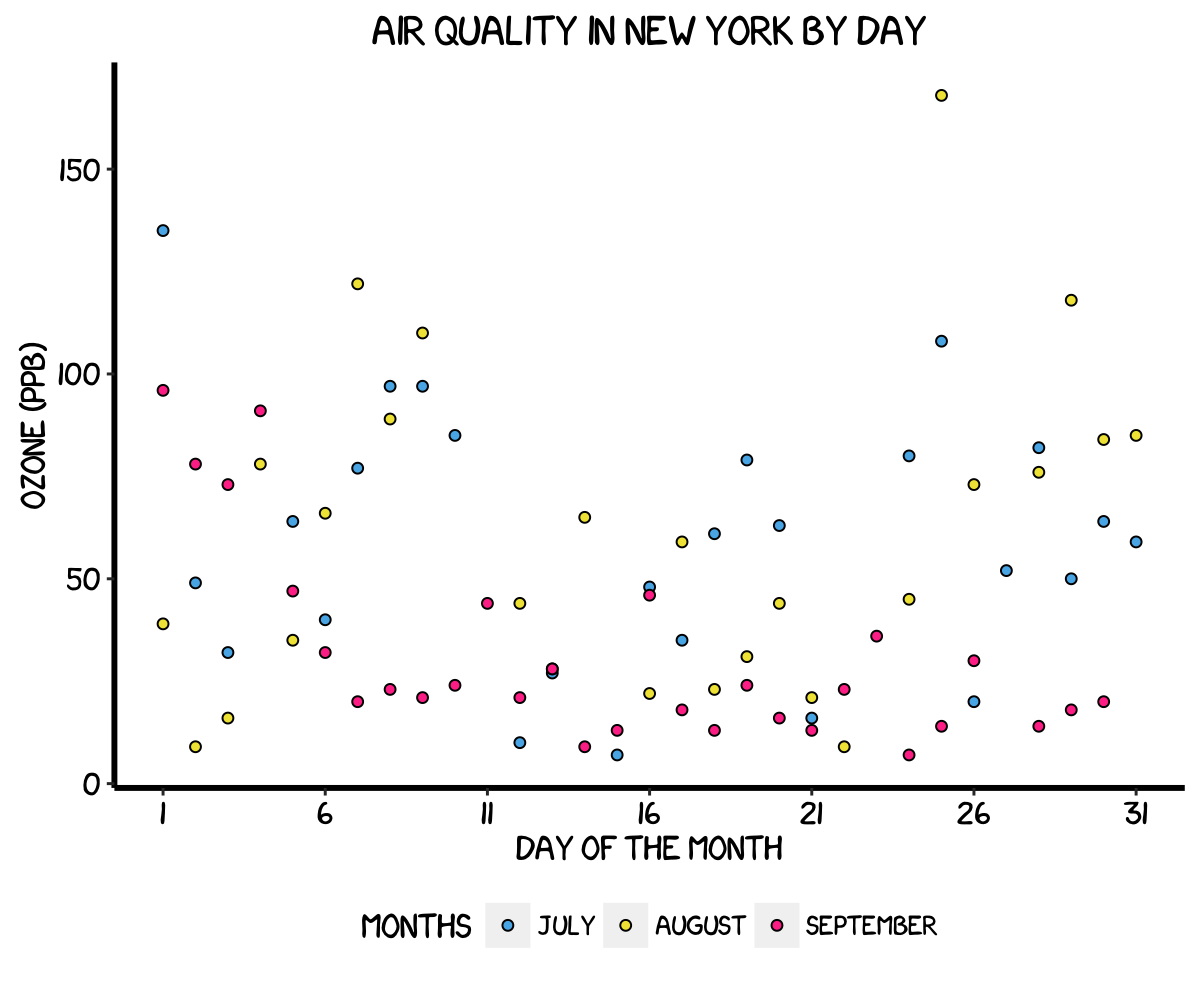
\includegraphics[width=0.55\linewidth]{0_all_posts_pdf/scatter_13-1} \end{center}

\section{\texorpdfstring{Using `The Economist'
theme}{Using The Economist theme}}\label{using-the-economist-theme-4}

There are a wider range of pre-built themes available as part of the
\texttt{ggthemes} package (more information on these
\href{https://cran.r-project.org/web/packages/ggthemes/vignettes/ggthemes.html}{here}).
Below we've applied \texttt{theme\_economist()}, which approximates
graphs in the Economist magazine.

\begin{Shaded}
\begin{Highlighting}[]
\NormalTok{p5 <-}\StringTok{ }\KeywordTok{ggplot}\NormalTok{(aq_trim, }\KeywordTok{aes}\NormalTok{(}\DataTypeTok{x =} \NormalTok{Day, }\DataTypeTok{y =} \NormalTok{Ozone, }\DataTypeTok{fill =} \NormalTok{Month)) +}
\StringTok{      }\KeywordTok{scale_fill_economist}\NormalTok{() +}
\StringTok{      }\KeywordTok{geom_point}\NormalTok{(}\DataTypeTok{shape =} \DecValTok{21}\NormalTok{) +}
\StringTok{      }\KeywordTok{ggtitle}\NormalTok{(}\StringTok{"Air Quality in New York by Day"}\NormalTok{) +}\StringTok{ }
\StringTok{      }\KeywordTok{labs}\NormalTok{(}\DataTypeTok{x =} \StringTok{"Day of the month"}\NormalTok{, }\DataTypeTok{y =} \StringTok{"Ozone (ppb)"}\NormalTok{, }\DataTypeTok{fill =} \StringTok{"Months"}\NormalTok{) +}
\StringTok{      }\KeywordTok{scale_x_continuous}\NormalTok{(}\DataTypeTok{breaks =} \KeywordTok{seq}\NormalTok{(}\DecValTok{1}\NormalTok{, }\DecValTok{31}\NormalTok{, }\DecValTok{5}\NormalTok{)) +}
\StringTok{      }\KeywordTok{scale_size}\NormalTok{(}\DataTypeTok{range =} \KeywordTok{c}\NormalTok{(}\DecValTok{1}\NormalTok{, }\DecValTok{10}\NormalTok{)) +}
\StringTok{      }\KeywordTok{theme_economist}\NormalTok{() +}\StringTok{ }
\StringTok{      }\KeywordTok{theme}\NormalTok{(}\DataTypeTok{axis.line.x =} \KeywordTok{element_line}\NormalTok{(}\DataTypeTok{size=}\NormalTok{.}\DecValTok{5}\NormalTok{, }\DataTypeTok{colour =} \StringTok{"black"}\NormalTok{), }
\StringTok{        }\DataTypeTok{axis.line.y =} \KeywordTok{element_line}\NormalTok{(}\DataTypeTok{size=}\NormalTok{.}\DecValTok{5}\NormalTok{, }\DataTypeTok{colour =} \StringTok{"black"}\NormalTok{), }
\StringTok{        }\DataTypeTok{axis.title =} \KeywordTok{element_text}\NormalTok{(}\DataTypeTok{size =} \DecValTok{12}\NormalTok{),}
\StringTok{        }\DataTypeTok{legend.position =} \StringTok{"bottom"}\NormalTok{, }\DataTypeTok{legend.direction =} \StringTok{"horizontal"}\NormalTok{,}
\StringTok{        }\DataTypeTok{legend.text =} \KeywordTok{element_text}\NormalTok{(}\DataTypeTok{size =} \DecValTok{9}\NormalTok{),}
\StringTok{        }\DataTypeTok{legend.title=}\KeywordTok{element_text}\NormalTok{(}\DataTypeTok{face =} \StringTok{"bold"}\NormalTok{, }\DataTypeTok{size =} \DecValTok{9}\NormalTok{),}
\StringTok{        }\DataTypeTok{text =} \KeywordTok{element_text}\NormalTok{(}\DataTypeTok{family =} \StringTok{"Tahoma"}\NormalTok{),  }
\StringTok{        }\DataTypeTok{plot.title =} \KeywordTok{element_text}\NormalTok{(}\DataTypeTok{family=}\StringTok{"Tahoma"}\NormalTok{))}
\NormalTok{p5}
\end{Highlighting}
\end{Shaded}

\begin{center}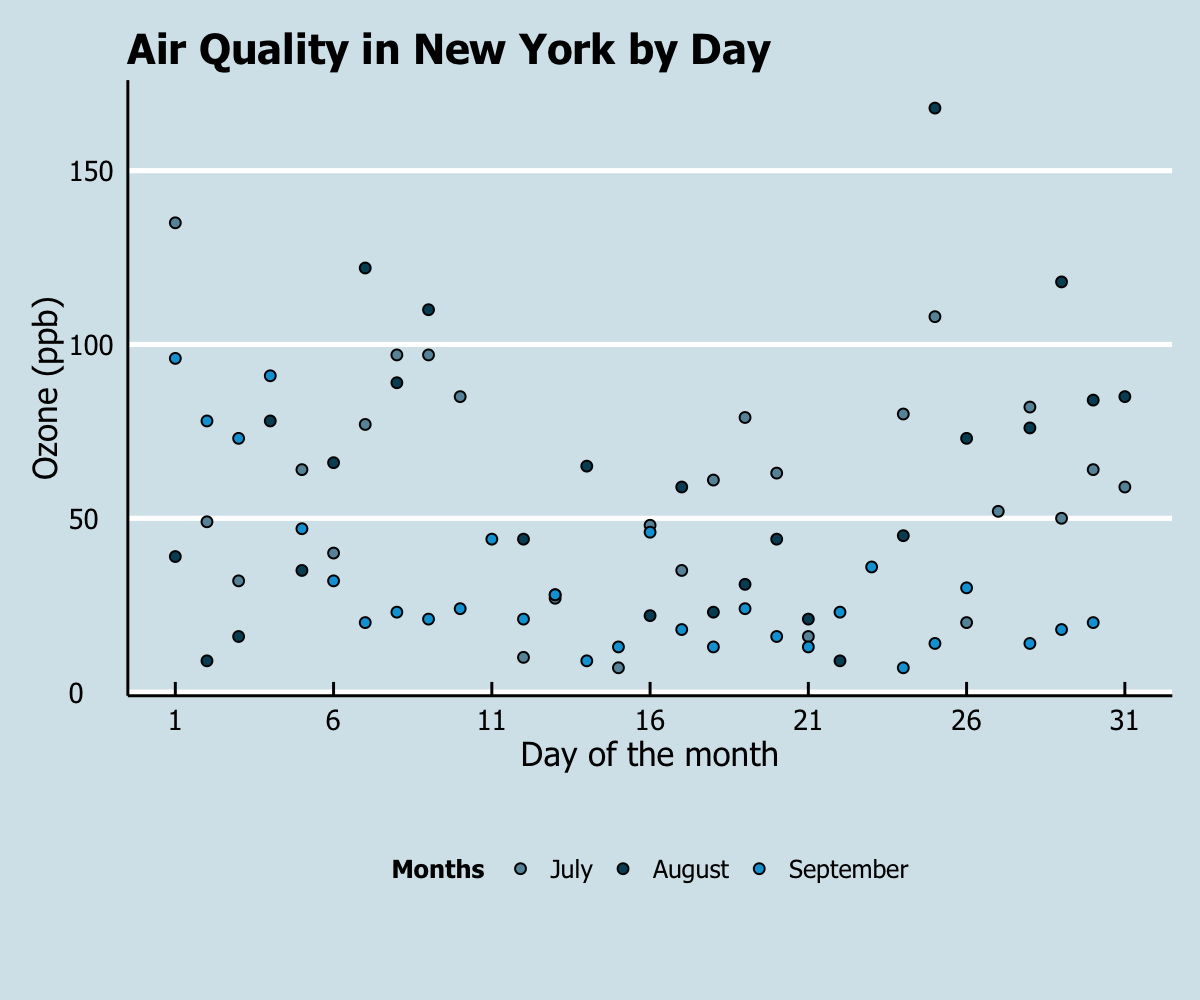
\includegraphics[width=0.55\linewidth]{0_all_posts_pdf/scatter_14-1} \end{center}

\section{Creating your own theme}\label{creating-your-own-theme-4}

As before, you can modify your plots a lot as \texttt{ggplot2} allows
many customisations. Here we present our original result shown at the
top of page.

\begin{Shaded}
\begin{Highlighting}[]
\NormalTok{fill =}\StringTok{ }\KeywordTok{c}\NormalTok{(}\StringTok{"steelblue"}\NormalTok{, }\StringTok{"yellowgreen"}\NormalTok{, }\StringTok{"violetred1"}\NormalTok{)}

\NormalTok{p5 <-}\StringTok{ }\KeywordTok{ggplot}\NormalTok{(aq_trim, }\KeywordTok{aes}\NormalTok{(}\DataTypeTok{x =} \NormalTok{Day, }\DataTypeTok{y =} \NormalTok{Ozone, }\DataTypeTok{fill =} \NormalTok{Month)) +}
\StringTok{      }\KeywordTok{geom_point}\NormalTok{(}\DataTypeTok{shape =} \DecValTok{21}\NormalTok{) +}
\StringTok{      }\KeywordTok{ggtitle}\NormalTok{(}\StringTok{"Air Quality in New York by Day"}\NormalTok{) +}\StringTok{ }
\StringTok{      }\KeywordTok{labs}\NormalTok{(}\DataTypeTok{x =} \StringTok{"Day of the month"}\NormalTok{, }\DataTypeTok{y =} \StringTok{"Ozone (ppb)"}\NormalTok{, }\DataTypeTok{fill =} \StringTok{"Months"}\NormalTok{) +}
\StringTok{      }\KeywordTok{scale_x_continuous}\NormalTok{(}\DataTypeTok{breaks =} \KeywordTok{seq}\NormalTok{(}\DecValTok{1}\NormalTok{, }\DecValTok{31}\NormalTok{, }\DecValTok{5}\NormalTok{)) +}
\StringTok{      }\KeywordTok{scale_size}\NormalTok{(}\DataTypeTok{range =} \KeywordTok{c}\NormalTok{(}\DecValTok{1}\NormalTok{, }\DecValTok{10}\NormalTok{)) +}
\StringTok{      }\KeywordTok{scale_fill_manual}\NormalTok{(}\DataTypeTok{values =} \NormalTok{fill) +}
\StringTok{      }\KeywordTok{theme}\NormalTok{(}\DataTypeTok{axis.line.x =} \KeywordTok{element_line}\NormalTok{(}\DataTypeTok{size=}\DecValTok{1}\NormalTok{, }\DataTypeTok{colour =} \StringTok{"black"}\NormalTok{), }
\StringTok{        }\DataTypeTok{axis.line.y =} \KeywordTok{element_line}\NormalTok{(}\DataTypeTok{size=}\DecValTok{1}\NormalTok{, }\DataTypeTok{colour =} \StringTok{"black"}\NormalTok{), }
\StringTok{        }\DataTypeTok{axis.text.x=}\KeywordTok{element_text}\NormalTok{(}\DataTypeTok{colour=}\StringTok{"black"}\NormalTok{, }\DataTypeTok{size =} \DecValTok{9}\NormalTok{), }
\StringTok{        }\DataTypeTok{axis.text.y=}\KeywordTok{element_text}\NormalTok{(}\DataTypeTok{colour=}\StringTok{"black"}\NormalTok{, }\DataTypeTok{size =} \DecValTok{9}\NormalTok{),  }
\StringTok{        }\DataTypeTok{legend.position =} \StringTok{"bottom"}\NormalTok{, }\DataTypeTok{legend.direction =} \StringTok{"horizontal"}\NormalTok{,}
\StringTok{        }\DataTypeTok{panel.grid.major =} \KeywordTok{element_line}\NormalTok{(}\DataTypeTok{colour =} \StringTok{"#d3d3d3"}\NormalTok{), }
\StringTok{        }\DataTypeTok{panel.grid.minor =} \KeywordTok{element_blank}\NormalTok{(), }
\StringTok{        }\DataTypeTok{panel.border =} \KeywordTok{element_blank}\NormalTok{(), }\DataTypeTok{panel.background =} \KeywordTok{element_blank}\NormalTok{(),}
\StringTok{        }\DataTypeTok{plot.title =} \KeywordTok{element_text}\NormalTok{(}\DataTypeTok{size =} \DecValTok{14}\NormalTok{, }\DataTypeTok{family =} \StringTok{"Tahoma"}\NormalTok{, }
\StringTok{        }\DataTypeTok{face =} \StringTok{"bold"}\NormalTok{),}
\StringTok{        }\DataTypeTok{text=}\KeywordTok{element_text}\NormalTok{(}\DataTypeTok{family=}\StringTok{"Tahoma"}\NormalTok{)) }
\NormalTok{p5}
\end{Highlighting}
\end{Shaded}

\begin{center}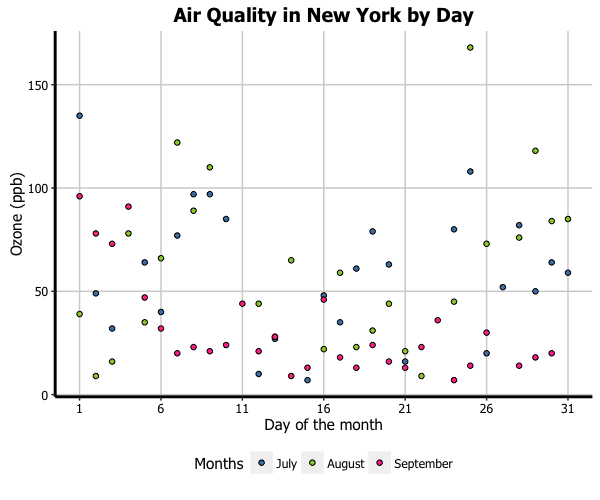
\includegraphics[width=0.55\linewidth]{0_all_posts_pdf/scatter_15-1} \end{center}